%!TEX root = ../main.tex

\chapter{Invio dei dati al satellite}

Per inviare i dati al satellite le informazioni sono codificate nelle onde elettromagnetiche attraverso un processo chiamato modulazione.
Tutte le informazioni trasmesse attraverso un mezzo di comunicazione senza fili sono modulate in qualche modo.
Il criterio principale per la scelta dello schema di modulazione è basato sulla massimizzazione del data rate e minimizzazione della potenza trasmessa, della larghezza di banda del canale, dell'errore sul simbolo e resistenza alle interferenze.

Le tecniche di modulazione e demodulazione digitale richiedono una maggiore complessità e un elevato livello di integrazione per trasferire grandi quantità di dati e informazioni.
Un filtraggio eccessivo per migliorare l'efficienza spettrale può ridurre le interferenze ma aumentare il \ac{BER} (Bit Error Rate) a causa della sfocatura dei simboli trasmessi.

Per inviare dati digitali usando una tecnologia analogica, l'emittente genera un sengale portante a una certa frequenza.
Per codificare il segnale digitale nella sinusoide sono poi utilizzate le seguenti tecniche:
\begin{itemize}
  \item Amplitude-shift modulation (keying): varia l'ampiezza (cioè la tensione) del segnale.
  \item Frequency-shift modulation: due (o più) frequenze vicine alla frequenza portante sono utilizzate.
  \item Phase-shift modulation: sposta sistematicamente l'onda portante a intervalli uniformemente spaziati.
\end{itemize}

Oltre alla modulazione i dati vengono trasmessi efficientemente anche utilizzando tecniche di multiplexing.
Il multiplexing consente di combinare più sengali in un singolo canale di trasmissione, massimizzando l'uso della banda e migliorando l'efficienza del sistema.
Esistono due principali approcci al multiplexing: FDM (Frequency Division Multiplexing) e TDM (Time Division Multiplexing).
L'FDM suddivide lo spettro di frequenza in sottocanali, dando a ciascun utente l'utilizzo esclusivo di un sottocanale.
Un problema con FDM è che a un utente è data tutta la frequenza, e se non ha dati da inviare la banda è sprecata, dato che non può essere utilizzata da un altro utente.
Il TDM invece utilizza il time slicing per dare a ciascun utente l'intera banda, ma solo per una frazione di secondo alla volta.
Di nuovo, se l'utente non ha dati da inviare durante il suo timeslice, la banda non è utilizzata, e quindi è sprecata.


% AGGIUNGERE
% COMPARISON OF ADVANCED CODING AND MODULATION SCHEMES FOR MULTICARRIER SATELLITE COMMUNICATION SYSTEMS
% SATELLITE COMMUNICATION MODULATION TECHNIQUES IMPLEMENTED USING SIMULINK AND MATLAB
%

La capacità di un satellite Starlink sarà di 20 Gbit/s quando opererà in due polarizzazioni con modulazione 64-\ac{QAM}.
Ad oggi la rete può usare solo una polarizzazione.
Per lavorare con la 64-\ac{QAM} è necessario avere un \ac{SNR} di più di 17dB.
Al momento questo parametro al terminale UT-1 è tra gli 11 e i 12.5 dB, che corrisponde a una 16-32\ac{APSK} e ha un'efficienza spettrale di 4.5 bit/s/Hz al massimo.
Le possibili efficienze spettrali per Starlink sono:

\begin{table}[h]
\centering
\begin{tabular}{|c|c|c|c|}
\hline
\textbf{Modulation} & \textbf{Code rate} & \makecell{\textbf{Spectral efficiency}\\ \textbf{bit/s/Hz}} \\ \hline
QPSK     & 0.5   & 0.989  \\ \hline
8PSK     & 0.75  & 2.228  \\ \hline
8PSK     & 0.833 & 2.479  \\ \hline
16APSK   & 0.666 & 2.637  \\ \hline
16APSK   & 0.75  & 2.967  \\ \hline
32APSK   & 0.9   & 4.453  \\ \hline
64QAM    & 0.772 & 4.5234 \\ \hline
64QAM    & 0.873 & 5.1152 \\ \hline
64QAM    & 0.948 & 5.5547 \\ \hline
\end{tabular}
\caption{Efficienza spettrale di Starlink \cite{rozenvasser_estimation_2023}}
\end{table}

\paragraph{Link budget}
La potenza ricevuta al terminale utente è data da:
\begin{equation}
P_{rx} = P_{tx} + G_{tx} + G_{rx} - L_{tx} - L_{rx} - L_{atm} - L_{p}
\label{eq:received-power}
\end{equation}

In questa equazione, $P_{tx}$ è la potenza del trasmettitore, $G_{tx}$ e $G_{rx}$ sono i guadagni del trasmettitore e del ricevitore, $L_{tx}$ e $L_{rx}$ sono le perdite ai trasmettitori e ricevitori, $L_{atm}$ è la perdita atmosferica, e $L_{p}$ è il path loss introdotto dalla separazione tra il trasmettitore e il ricevitore.

% ROBA SENZA UN CAZZO DI SENSO

% $P_{tx}$ è la potenza del trasmettitore ed è dipendente dall'allocazione dinamica delle risorse $\eta_{a}$ e massa del satellite $m$.

% Il guadagno del trasmettitore $G_{tx}$ è dipendente dalla tecnologia dell'antenna (il diametro $d$ e la lunghezza d'onda $\lambda$):
% \begin{itemize}
%   \item Parabolica: $G_{tx} = 20 \log_{10} (\frac{\eta_{a} \pi d}{\lambda})$
%   \item Phased Array: $G_{tx} = 20 \log_{10} (\frac{4 \eta_{a} \pi \sqrt[3]{m^2}}{\lambda})$
% \end{itemize}

% Il guadagno del ricevitore sul rumore $G_{rx}$ basato sul tipo del terminale utente:
% \begin{itemize}
%   \item Parabolica: $G_{rx} = 5.24 dB$
%   \item Phased Array: $G_{rx} = 10.8 dB$
% \end{itemize}

La perdita atmosferica $L_{atm}$ è dipendente dalla banda di frequenza e pressione atmosferica $P_{atm}$.
Per la Ku/Ka-band $L_{atm} = 0.97 dB/km$ in media.

\begin{figure}[htbp]
  \centering
  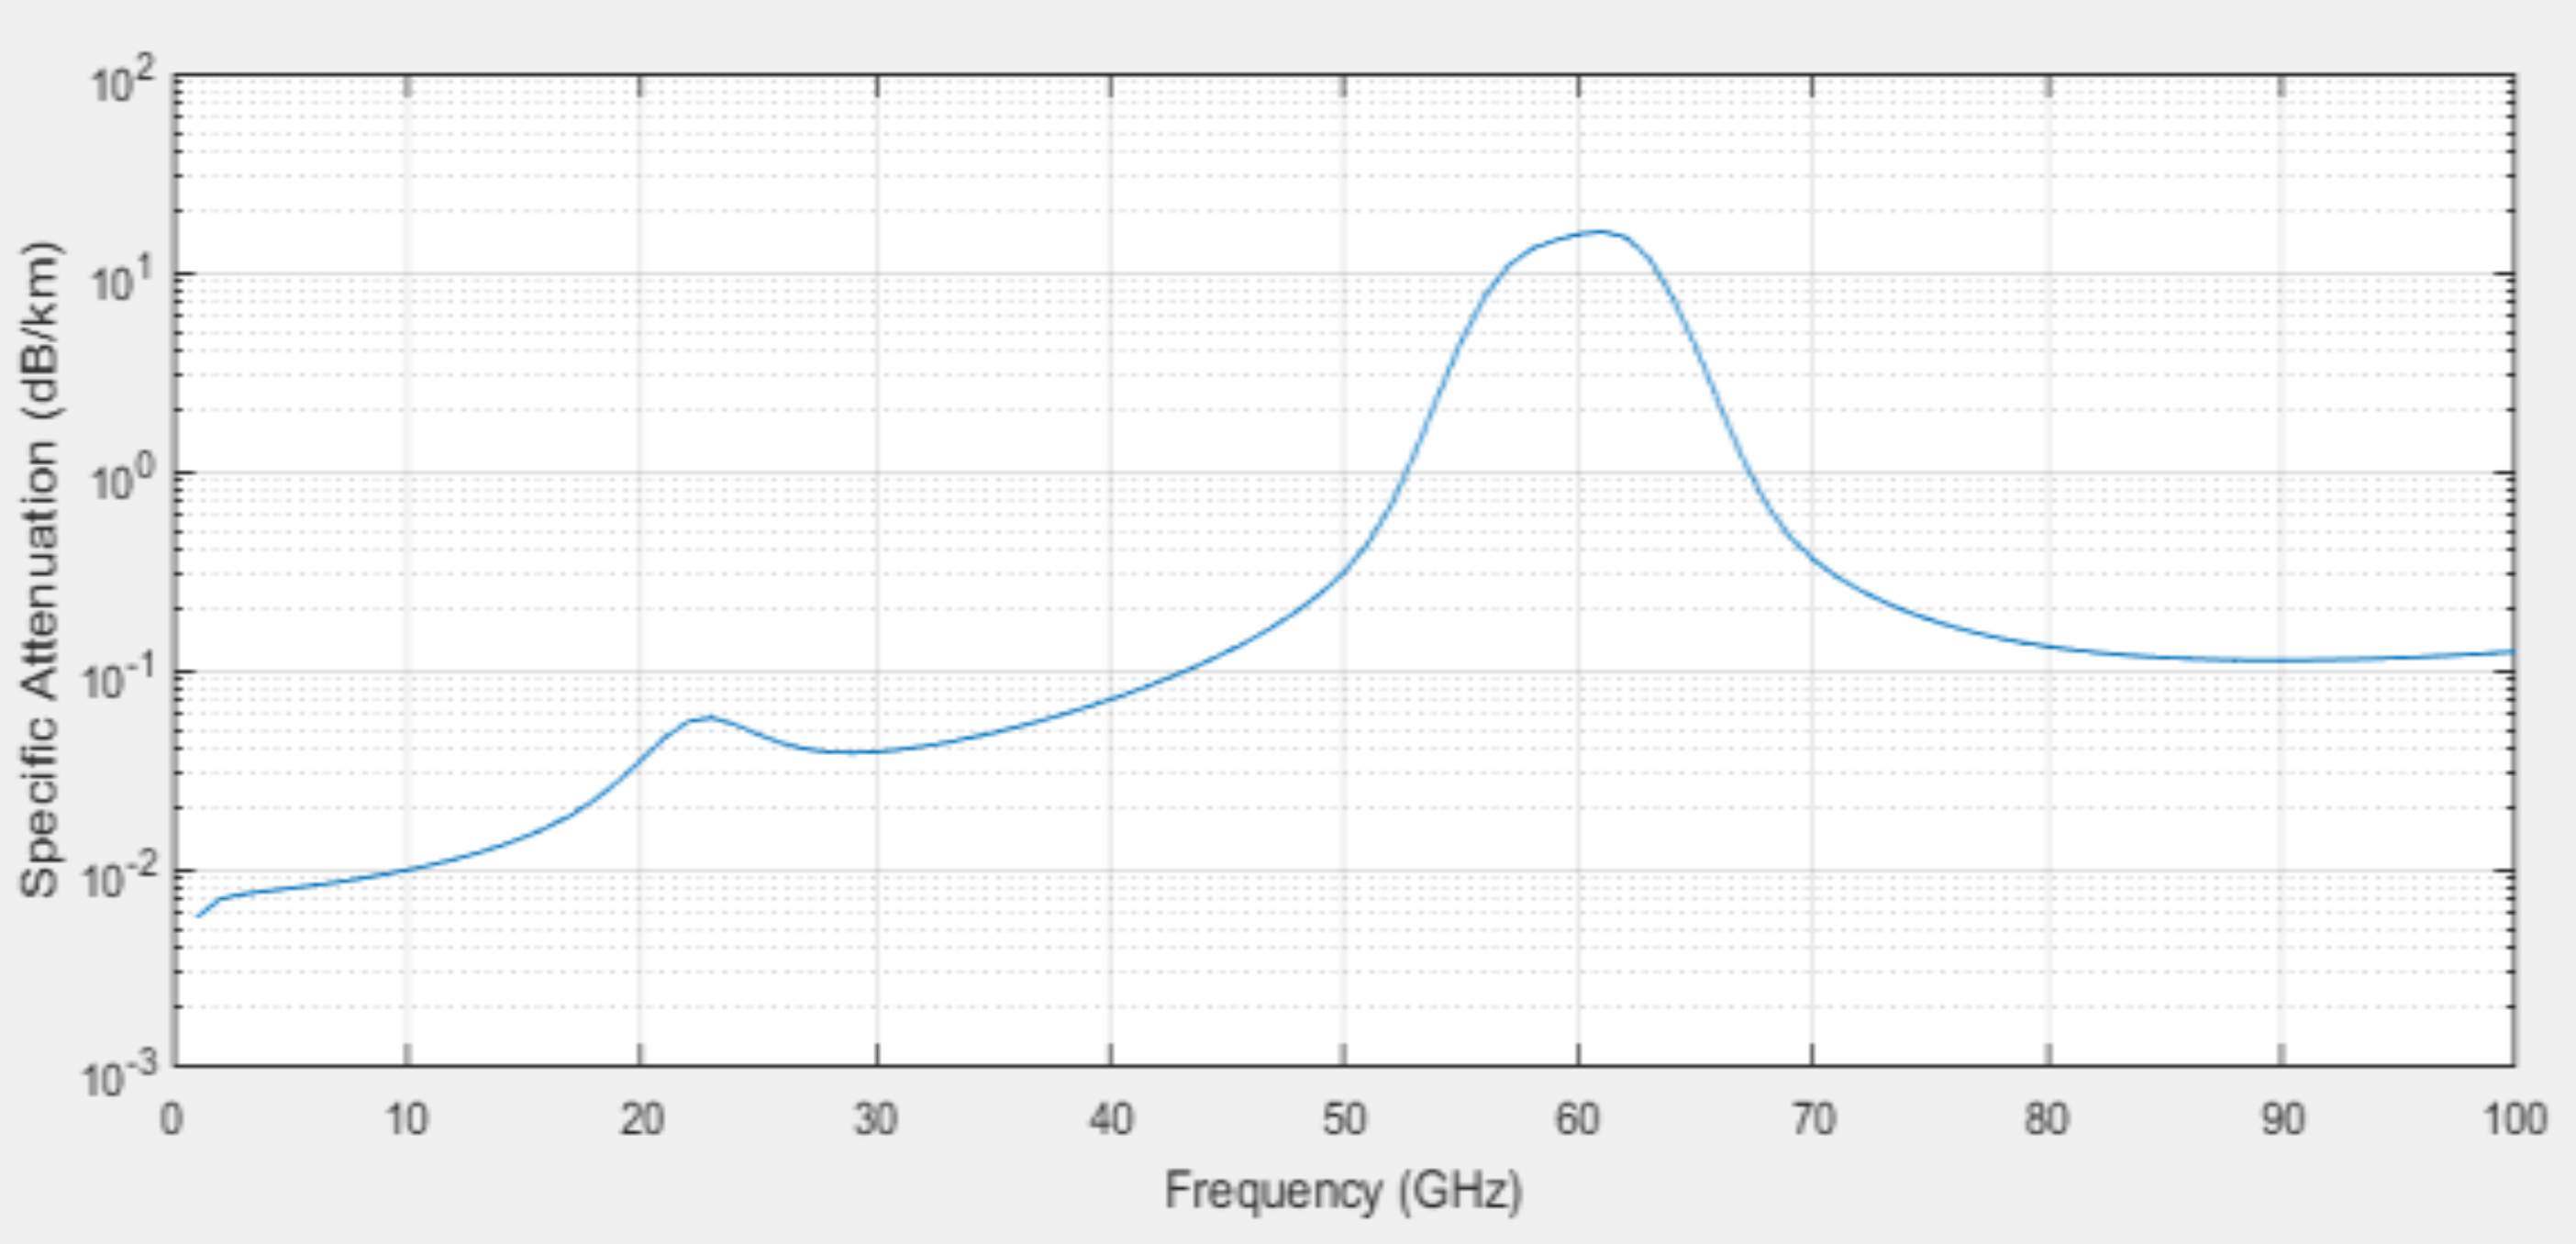
\includegraphics[width=0.8\linewidth]{./res/img/atmospheric_losses_simulation.png}
  \caption{Simulazione delle perdite atmosferiche}
  \label{fig:atmospheric-losses-simulation}
\end{figure}

Osserviamo in figura \ref{fig:atmospheric-losses-simulation} un picco del parametro $L_{atm}$ a 60 GHz.
Per ridurre l'influenza delle perdite atmosferiche è preferibile usare i range di frequenza fino a 53 GHz, che corrisponde al piano di frequenze proposto da SpaceX (tabella \ref{tab:starlink-frequency-allocation-modulation-type}).
Per la trasmissione in uplink si usano le frequenze 14-52.4 GHz e per la trasmissione in downlink le frequenze 10.7-42.5 GHz.
Nella tabella \ref{tab:starlink-frequency-allocation-modulation-type} possiamo anche vedere i tipi di modulazione.
Il tipo di modulazione può cambiare da \ac{BPSK} a 64-\ac{QAM}.

\begin{table}[h]
\centering
\begin{tabular}{|c|c|c|}
\hline
\textbf{Caratteristica} & \textbf{Uplink} & \textbf{Downlink} \\ \hline
Frequenza (GHz)  & \makecell{14.0-14.5 \\ 27.5-29.1 \\ 29.5-30.0 \\ 47.2-52.4}  & \makecell{10.7-12.7\\17.8-18.6\\18.8-19.3\\37.5-42.5} \\ \hline
Tipo di modulazione  & \makecell{\acs{BPSK},\\M\acs{QAM}} & \makecell{\acs{OQPSK},\\ M\acs{QAM}} \\ \hline
\end{tabular}
\caption{Path loss nello spazio aperto in dB ($L_p$) \cite{rozenvasser_estimation_2023}.}
\label{tab:starlink-frequency-allocation-modulation-type}
\end{table}

% $L_p = 20 \log_{10} (\frac{4 \pi d}{\lambda})$

\begin{figure}[htbp]
  \centering
  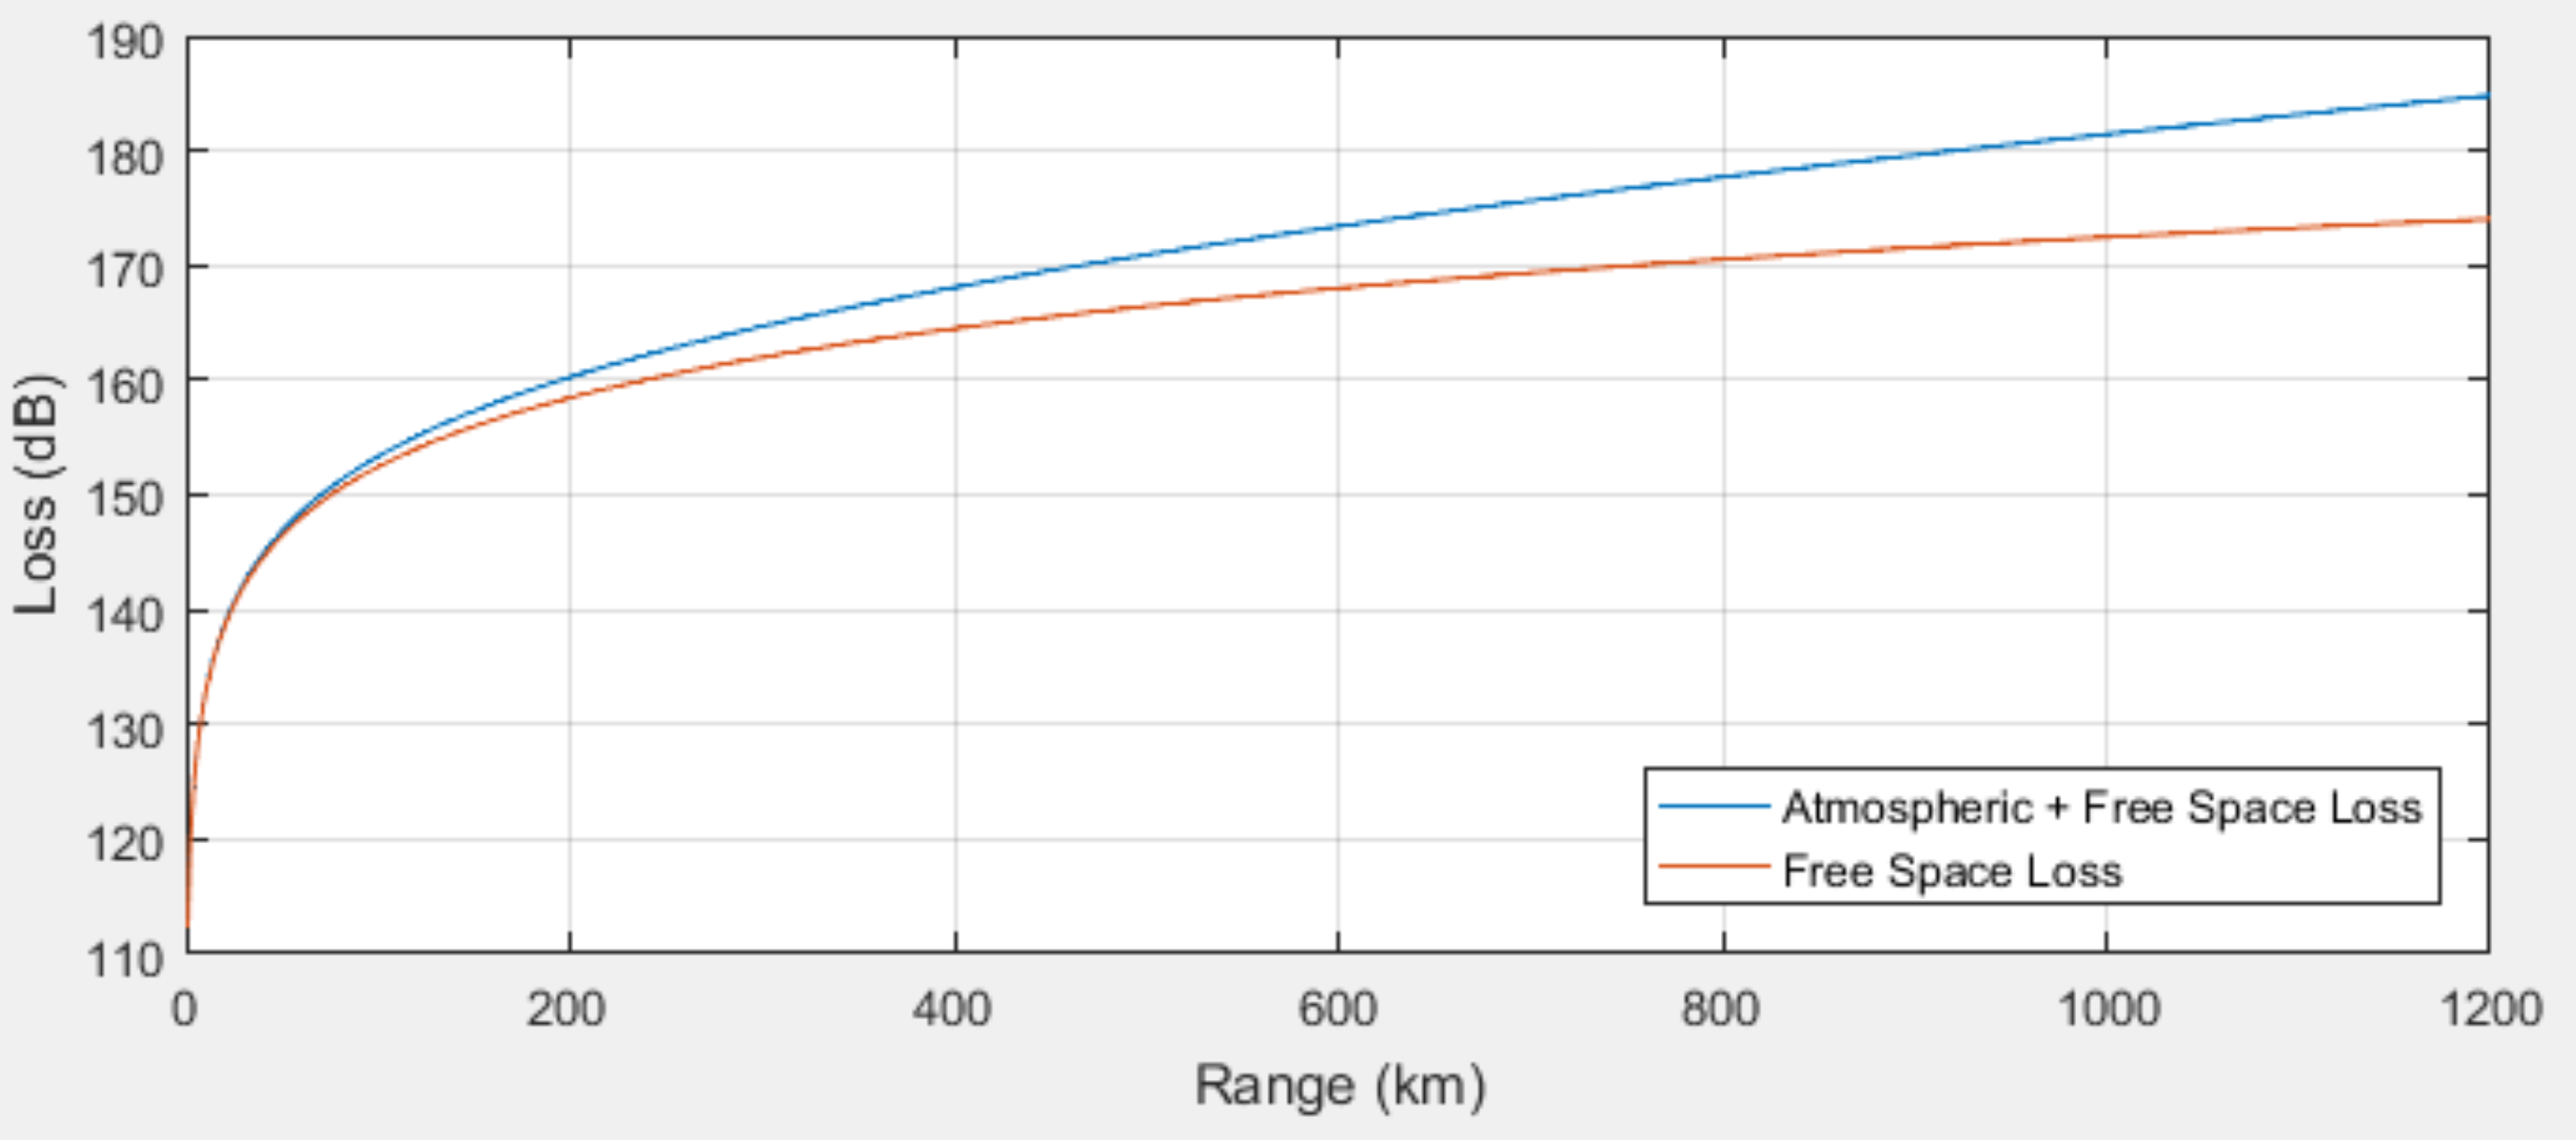
\includegraphics[width=0.8\linewidth]{./res/img/free_space_path_loss_atm_loss.png}
  \caption{Path loss nello spazio libero e perdita atmosferica}
  \label{fig:free-space-path-loss-atm-loss}
\end{figure}

Il path loss nello spazio libero è il contributore principale alla perdita di potenza come si vede in figura \ref{fig:free-space-path-loss-atm-loss}.
Alle altitudini calcolate per i satelliti Starlink, questo valore è di 160-175 dB.
La perdita totale dal path loss nello spazio libero e le perdite atmosferiche sono 165-185 dB.

I risultati della modellazione e del calcolo della dipendenza della potenza ricevuta dal terminale utente dall'altezza dell'orbita del satellite per varie frequenze (da 10 a 50 GHz) sono illustrati nella figura \ref{fig:link-budget-wo-ecc}.

\begin{figure}[htbp]
  \centering
  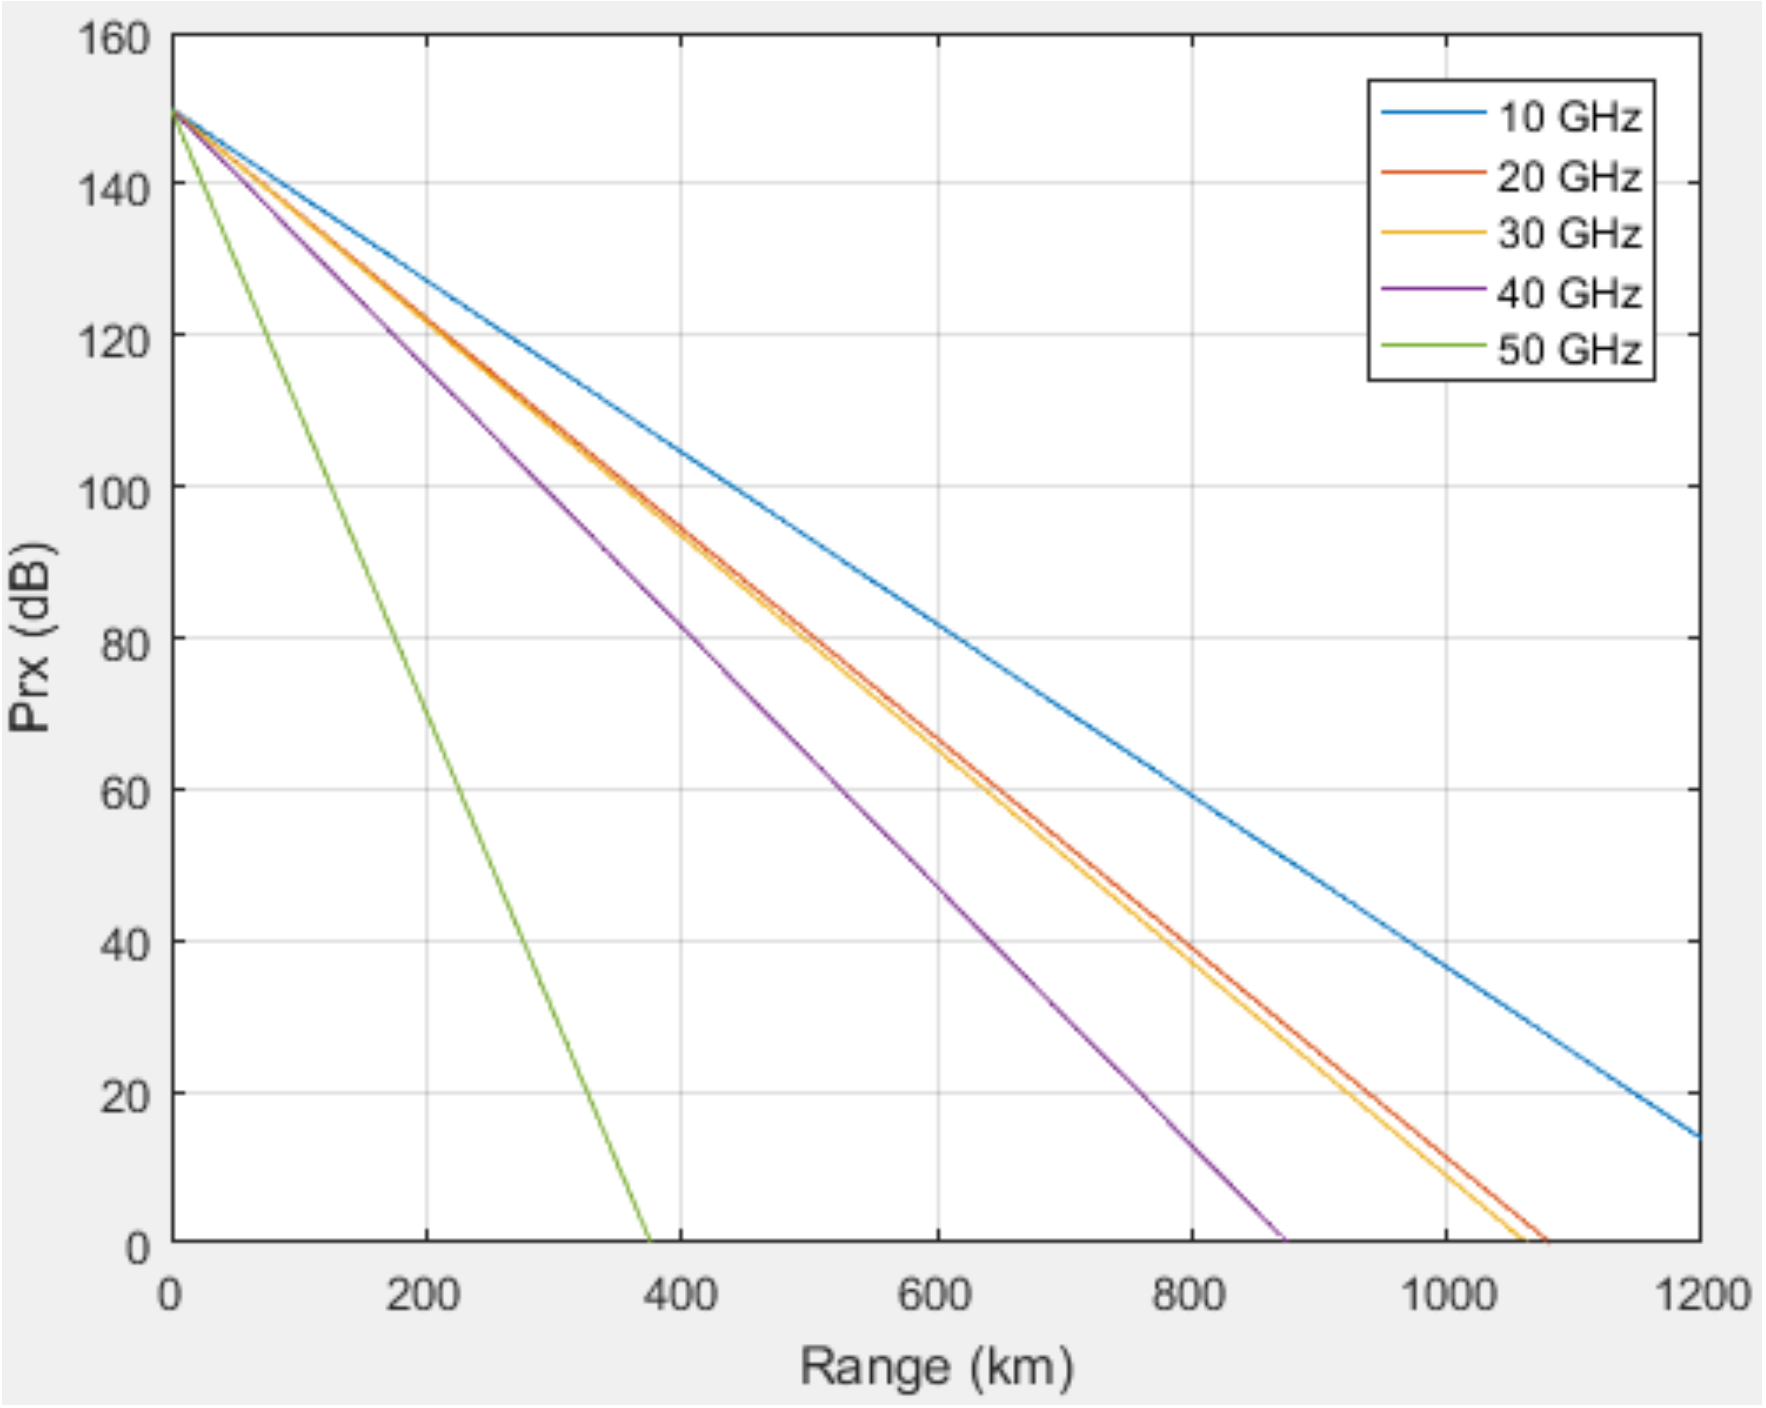
\includegraphics[width=0.8\linewidth]{./res/img/link_budget_wo_ecc.png}
  \caption{Link budget senza \ac{ECC}}
  \label{fig:link-budget-wo-ecc}
\end{figure}

Dalla figura \ref{fig:link-budget-wo-ecc} si può vedere che il valore più alto della potenza del segnale è 150 dB.
Finchè il segnale passa attraverso l'atmosfera gradualmente viene attenuato.
L'attenuazione avviene anche sui dispositivi ricevitori e trasmettitori.
Il grado di attenuazione dipende da molti parametri e limita l'altezza dell'orbita del satellite.

È consuetudine utilizzare un codice a correzione di errore per aumentare l'immunità al rumore dei sistemi.
In questo caso, utilizziamo un codice a correzione di errore per aumentare il link budget.

Aggiungiamo CG, guadagno di codifica dovuto al codice a correzione d'errore (\ac{ECC}), all'equazione (\ref{eq:received-power}) che diventa quindi:

\begin{equation}
  P_{rx} = P_{tx} + G_{tx} + G_{rx} - L_{tx} - L_{rx} - L_{atm} - L_{p} + CG
\end{equation}

I risultati della modellazione e calcolo della dipendenza della potenza ricevuta al terminale utente all'altezza dell'orbita del satellite per frequenze diverse (dai 10 ai 50 GHz), considerando l'uso di un codice di correzione di errore con un guadagno di codice di 10 dB sono mostrate in figura \ref{fig:link-budget-w-ecc}.

\begin{figure}[htbp]
  \centering
  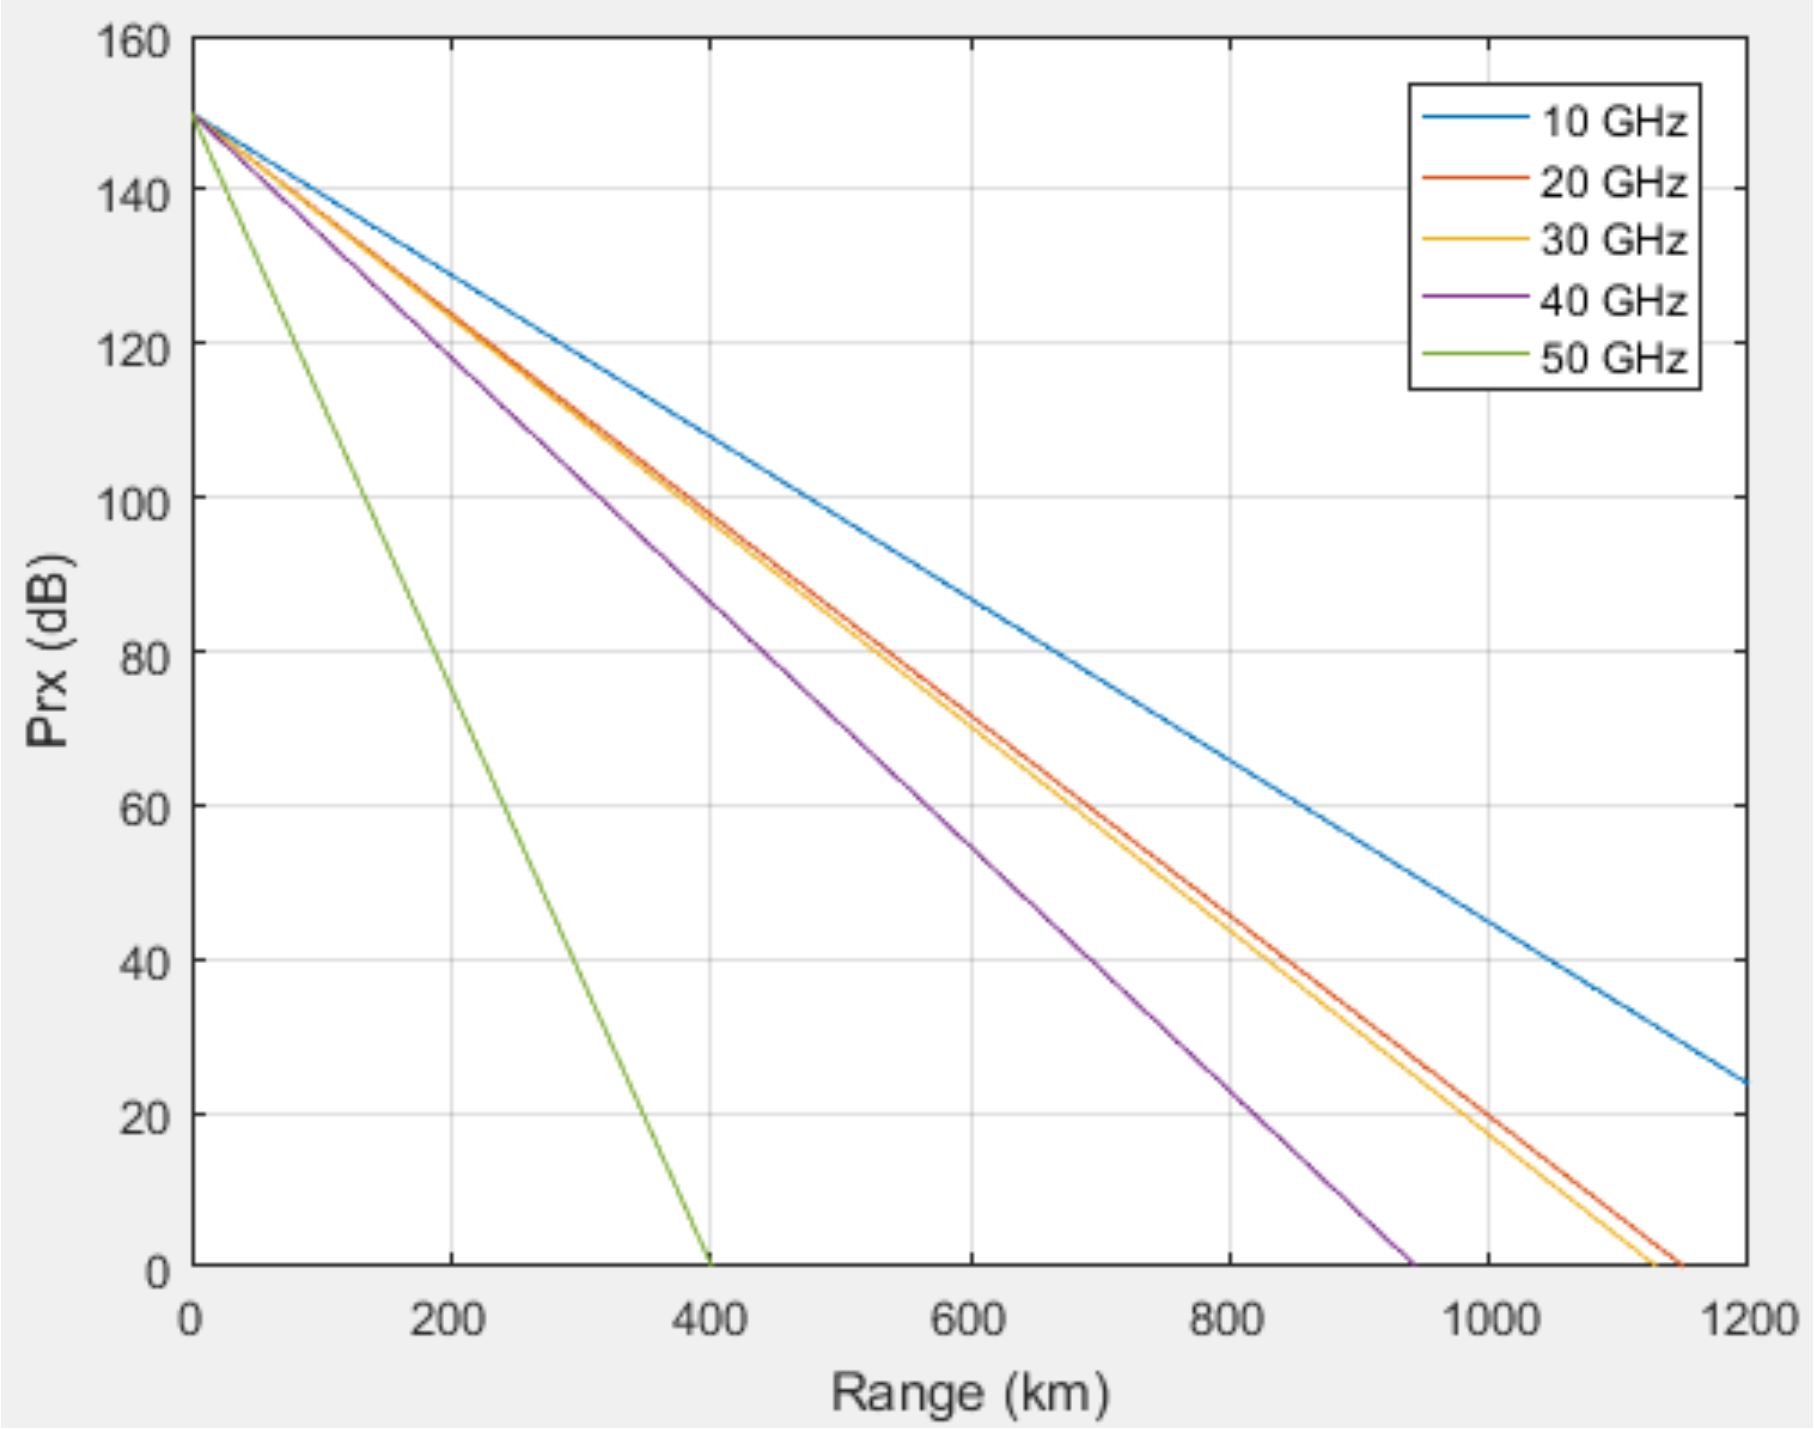
\includegraphics[width=0.8\linewidth]{./res/img/link_budget_w_ecc.png}
  \caption{Link budget con \ac{ECC}}
  \label{fig:link-budget-w-ecc}
\end{figure}

Per assicurare la minima probabilità d'errore è necessario avere un margine del \ac{SNR} al ricevitore, che dipende dal tipo di modulazione.
Dalla figura \ref{fig:link-budget-w-ecc} possiamo vedere che ad alte frequenze l'altezza dell'oribita è limitata a 340 km.
Il lancio della maggior parte dei satelliti è pianificata a quest'altezza.
Per frequenze più basse, possono essere utilizzate orbite più alte a 550 km e 1110 km \cite{rozenvasser_estimation_2023}.

\section{Direzionamento del traffico}
Starlink direziona il traffico dai terminali utenti alle ground station in un processo a due step.

\begin{figure}[htbp]
  \centering
  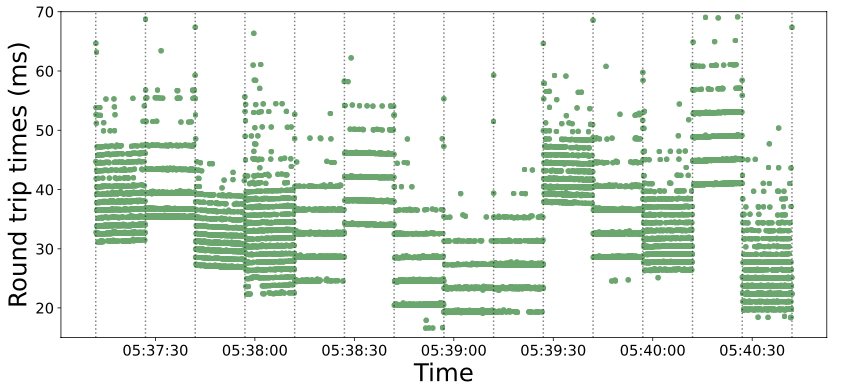
\includegraphics[width=0.8\linewidth]{./res/img/rtt_euterminal.png}
  \caption{\ac{RTT} misurato da un terminale in Europa \cite{tanveer_making_2023}}
  \label{fig:rtt-euterminal}
\end{figure}

Da come si può vedere in figura \ref{fig:rtt-euterminal} i cambiamenti di latenza misurati avvengono ogni 15 secondi.
Questo viene fatto da un controller globale, che alloca i satelliti ai terminali utenti basandosi su fattori quali il carico (inteso come banda del satellite occupata da altri utenti), condizioni geospaziali (principalmente visibilità del satellite dal terminale utente e condizioni atmosferiche), e carica del satellite.

C'è anche un controller nel satellite, che pianifica i flussi dai terminali utente assegnati a un satellite specifico.
Questo si può notare dalla presenza di bande di latenza parallele negli intervalli di 15 secondi di allocazione dei terminali al satellite \cite{tanveer_making_2023}.
Misure successive hanno rivelato un alto jitter (varianza del ritardo della connessione) e packet loss rate dell'1-2\% non correlato con la congestione di rete.
Varianti tradizionali del \ac{TCP}, come Reno, faticano nell'ambiente delle comunicazioni satellitari, dato la soro sensibilità alla perdita di pacchetti e recupero lento del throughput.
Varianti moderne come CUBIC hanno performance migliori grazie al Selective Acknowledgement (SACK), che gli permette di differenziare packet loss isolati da una congestione di rete.
BBR, un algoritmo di controllo di congestione sviluppato da Google, ha dimostrato performance promettenti su Starlink mantenendo il tasso di invio anche durante la perdita di pacchetti.
L'algoritmo stima il prodotto banda-ritardo del percorso e aggiusta i tassi di invio basandosi sui cambiamenti di latenza.
Il problema di questo algoritmo è che la sua richiesta aggressiva di risorse può affamare le altre sessioni TCP \cite{geoff_huston_transport_2024}.

\subsection{Identificazioni delle allocazioni del satellite}
Per studiare l'algoritmo di scheduling, i ricercatori hanno dovuto identificare a quale satellite si connettevano i terminali utente.
Usando le mappe di ostruzione fornite dall'applicazione per smartphone di Starlink hanno usato una nuova tecnica per trovare la traiettoria dei satelliti a cui un terminale si è connesso di recente.
Il processo è sviluppato come segue:
\begin{enumerate}
  \item Estrarre le mappe di ostruzione 2D ogni 15 secondi usando \verb|starlink-grpc-tools| (che è una libreria per eseguire comandi su altri computer come se fossero eseguiti in locale) e ottenendo le posizioni dei satelliti disponibili pubblicamente.
  \item Allineare le mappe 2D con le mappe 3D nell'app di starlink per determinare i parametri delle mappe 2D, come centro, raggio, e la rappresentazione degli angoli di elevazione e azimuth.
  \item Isolare la traiettoria del satellite connesso durante uno slot di 15 secondi specifico facendo delle considerazioni sulle mappe di ostruzione dallo slot precedente e quello attuale.
  \item Identificare il satellite che serve il terminale utente comparando le traiettorie estratte con la posizione calcolata dei satelliti visibili usando la misura di distanza Dynamic Time Warping, che è un modo di confrontare due sequenze temporale che non sono perfettamente sincronizzate.
\end{enumerate}

\subsection{Caratteristiche e preferenze dello scheduler globale}
Le analisi dei satelliti allocati hanno rivelato diverse preferenze dello scheduler globale. Si possono individuare tre fattori determinanti per la scelta:
\begin{itemize}
  \item Posizione del satellite: lo scheduler preferisce satelliti con angoli di elevazione più alti, con la mediana dei satelliti selezionati a 22.9 gradi più alta di quelli non selezionati.
  Lo scheduler ha anche una preferenza per i satelliti a nord del terminale utente. Questo probabilmente è dovuto alla zona di esclusione dell'International Telecommunication Union per le orbite geostazionarie e considerazioni di efficienza energetica, dato che i satelliti con un angolo di elevazione più alto hanno bisogno di meno energia per la comunicazione.
  \item Data di lancio del satellite: lo scheduler dà priorità ai satelliti più nuovi, infatti la probabilità che un satellite sia selezionato aumenta all'aumentare della sua data di lancio. Questa preferenza potrebbe essere legata al mantenimento di una copertura stabile della costellazione, dato che i satelliti più vecchi stanno raggiungendo la fine del loro ciclo di vita.
  \item Stato di illuminazione: lo scheduler favorisce i satelliti illuminati dal sole, scegliendoli il 72.3\% delle volte quando sono disponibili sia satelliti illuminati che non. I satelliti non illuminati sono selezionati solo quando rappresentano almeno il 35\% dei satelliti disponibili. La scelta sembra comunque guidata dal fatto che il loro angolo di elevazione sia maggiore di quelli illuminati, probabilmente per risparmiare energia \cite{tanveer_making_2023}.
\end{itemize}

\section{Comparazione della struttura del segnale con sistemi terrestri OFDM}
La struttura del segnale inviato da Starlink utilizza \ac{OFDM}, una scelta popolare pre i sistemi di comunicazione wireless, come Wi-Fi e LTE.
Tuttavia, il progetto di starlink differisce dai sistemi usati sulla terra per diversi aspetti chiave, che riflettono le caratteristiche uniche del canale di comunicazione spazio-terra e gli obiettivi di Starlink.

\paragraph{Layout di canale} A differenza dei sistemi terresti dove la larghezza di banda e gli schemi di duplexing variano a livello regionale, Starlink impiega una struttura coerente per il downlink in banda Ku, con otto canali da 240 MHz separati da bande di guardia da 10 MHz.
Questa ampia banda di guardia consente di attivare più canali contemporaneamente all'interno di una cella di servizio e riduce al minimo le interferenze tra celle adiacenti.
In questo modo si riduce potenzialmente l'efficienza spettrale, ma si migliora l'affidabilità.

\paragraph{Layout dei frame}
I frame inviati da starlink, con un periodo di 1/750 secondi, seguono un layout consistenza con un'alta proporzione di sequenze di sincronizzazione; la PSS, SSS, CM1SS e CSS.
Questa enfasi sulla sincronizzazione, superiore a quella dell'LTE e di altri sistemi terrestri, consente un'accurata equalizzazione del canale e stima dell'effetto Doppler, migliorando potenzialmente l'affidabilita della comunicazione e consentendo un doppio uso per il PNT (Positioning Navigation e Timing).

\paragraph{Sequenze di sincronizzazione}
L'utilizzo di sequenze di sincronizzazione multiple per frame, includendo il PSS m-sequence-based e la 4-\ac{QAM}-modulated SSS, lo distingue dai tradizionali sistemi terresti.
L'utilizzo di queste sequenze di sincronizzazione e la scelta di un numero moderato di sottoportatori semplificano l'elaborazione del segnale e garantiscono una sincronizzazione robusta anche in condizioni difficili.

\paragraph{Efficienza e margini di design}
La struttura del segnale Starlink prioritizza l'affidabilità.
L'efficiente occupazione dei simboli OFDM sfrutta il basso ritardo del canale \ac{LEO}-terra.
Le ampie bande di guardia e l'elevata occupazione dei frame, pur riducendo l'efficienza spettrale, migliorano la mitigazione delle interferenze e la precisione della sincronizzazione.
La scelta di un numero relativamente basso di sottoportanti (N = 1024) indica un design che prioritizza la robustezza piuttosto che massimizzare il throughput teorico.

